\chapter{Foundation}

\section*{Introduction}
This chapter details the implementation phase of our project, which follows an agile methodology with four sprints. Each sprint focuses on delivering specific features and functionality according to the project backlog. The implementation utilizes a modern tech stack consisting of React \cite{ReactWebsite} with Vite \cite{ViteJSWebsite} for the frontend, Node.js \cite{NodeJSWebsite} with Express.js \cite{ExpressJSWebsite} for the backend, MySQL \cite{MySQLWebsite} for database management, and Tailwind CSS \cite{TailwindWebsite} for styling.

Our first sprint focused on establishing essential foundational components of the system, with the following key deliverables:

\subsection{Web Backoffice Authentication}
\begin{itemize}
    \item Admin dashboard login and authentication system
    \item Role-based access control for backoffice users (Super Admin, Admin, Agent)
    \item User management interface for creating and managing user accounts
    \item Permission management system for different user roles
    \item Security logs and audit trails for backoffice activities
    \item Session management and secure token handling
\end{itemize}

\section{Sprint 1: Authentication and User Management }
\subsection{Overview}
The first sprint focuses on establishing the core authentication system and user management functionality. This foundation is critical for all subsequent features as it defines user roles and access controls.

\subsection{User Types}
The system supports three distinct user types, each with different permissions and capabilities:
\begin{itemize}
    \item \textbf{Super Admin}: Has complete access to all system features and can manage admins and agents.
    \item \textbf{Admin}: Can manage agents and has access to administrative features within their assigned scope.
    \item \textbf{Agent}: Has limited access to the system based on their assigned responsibilities.
\end{itemize}


\subsection{Authentication System}
\subsubsection{Sign-up Process}
The sign-up process is illustrated in Figure \ref{fig:signup-diagram} below. The diagram shows the authentication flow for new users registering in the system.

\begin{figure}[ht!]
    \centering
    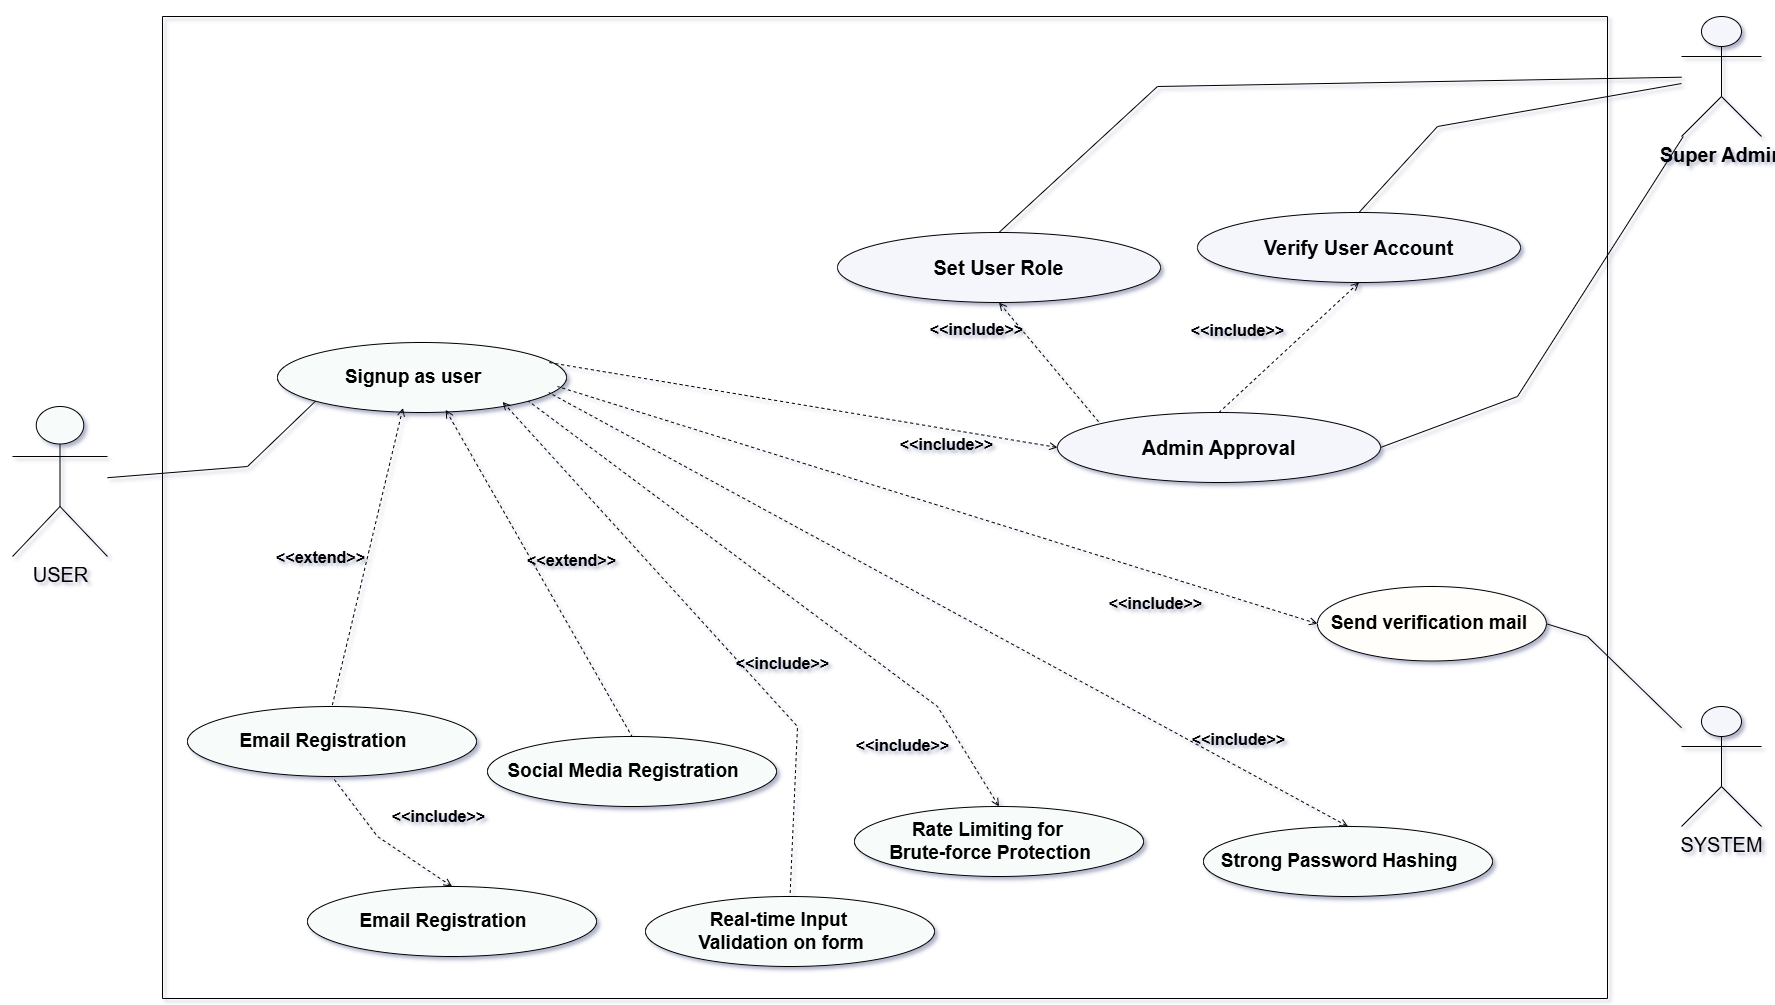
\includegraphics[width=1\textwidth]{images/diagram_de_case_d_utilisation_signup.png}
    \caption{Authentication Sign-up Use Case Diagram}
    \label{fig:signup-diagram}
\end{figure}

\newpage

\begin{figure}[ht!]
    \centering
    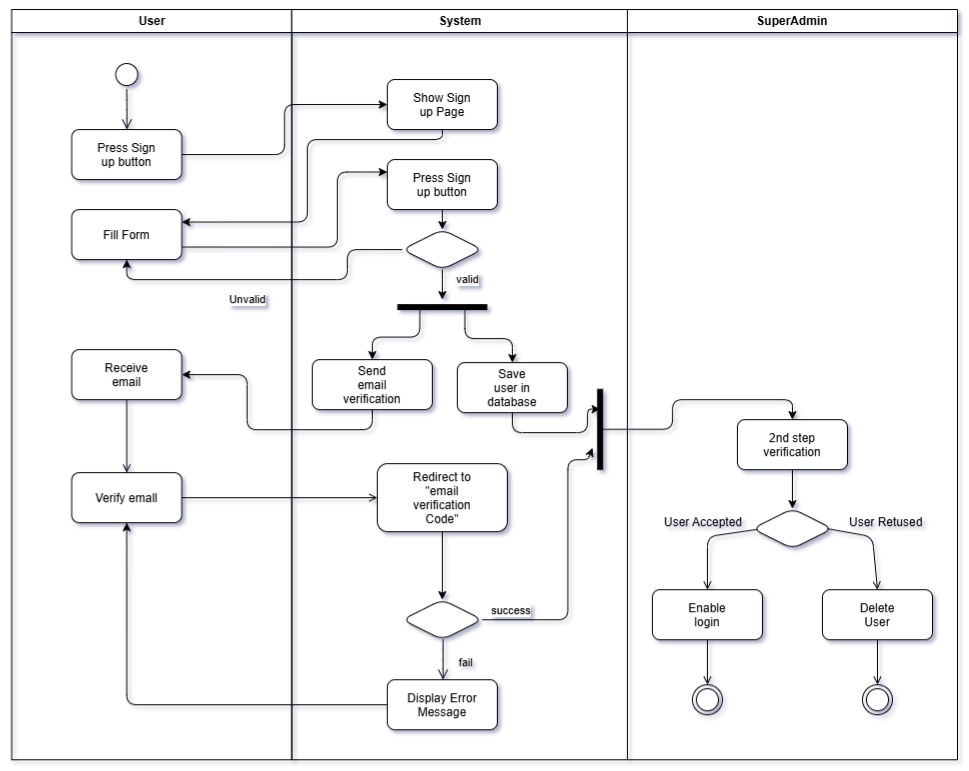
\includegraphics[width=1\textwidth]{images/signup_activitydiag.png}
    \caption{Authentication Sign-up Activity Diagram}
    \label{fig:signup-activity-diagram}
\end{figure}

Figure \ref{fig:signup-activity-diagram} illustrates the activity flow of the sign-up process. The process begins when a new user navigates to the sign-up page and presses the sign-up button. The system then presents a form for the user to fill out. Upon submission, the system validates the entered information. 

If the information is invalid, the user is prompted to correct the form. If the information is valid, the system saves the user's details in the database and sends a verification email to the user. The user must then check their email. 

Upon successful email verification, the system redirects the user to an "email verification code" page or a similar confirmation step. The Super Admin is then involved in a two-step verification process. If the Super Admin accepts the user, their login is enabled. If the Super Admin refuses the user, the user's account is deleted. If the initial email verification step fails (e.g., there's an issue with the verification code), an error message is displayed to the user.

% \vspace{1cm}

\subsubsection{Login Process}
The login process allows existing users to access the system. The table below details the use case.
\newpage
\begin{table}[htbp]
    \centering
    \begin{tabular}{|l|p{0.7\textwidth}|}
        \hline
        \textbf{Section} & \textbf{Details} \\
        \hline
        Use Case & User Login \\
        \hline
        Actor & User (Super Admin, Admin, Agent) \\
        \hline
        Precondition & User has an existing, verified account. User is on the login page. \\
        \hline
        Main Scenario & 
        1. User enters their credentials (e.g., email and password).
        2. User clicks the login button.
        3. System verifies the credentials.
        4. If credentials are valid, the system grants access and redirects the user to their respective dashboard. \\
        \hline
        Postcondition & User is successfully logged into the system and can access features based on their role. \\
        \hline
        Exception & 
        - Invalid credentials: System displays an error message.
        - Account locked/disabled: System displays an appropriate message.
        - System error: System displays a general error message. \\
        \hline
    \end{tabular}
    \caption{Login Process Details}
    \label{tab:login_process}
\end{table}

\subsubsection{Manage Users Process}
The user management process enables administrators to create, view, update, and delete user accounts. The table below details the use case.

\begin{table}[htbp]
    \centering
    \begin{tabular}{|l|p{0.7\textwidth}|}
        \hline
        \textbf{Section} & \textbf{Details} \\
        \hline
        Use Case & Manage User Accounts \\
        \hline
        Actor & Super Admin \\
        \hline
        Precondition & Actor is logged into the system with appropriate administrative privileges. \\
        \hline
        Main Scenario & 
        1. Actor navigates to the user management section.
        2. To create a user: Actor fills in user details (name, email, role, etc.) and submits the form. System creates the new user account.
        3. To view users: System displays a list of users. Actor can search/filter the list.
        4. To update a user: Actor selects a user, modifies their details, and saves the changes. System updates the user account.
        5. To delete a user: Actor selects a user and confirms deletion. System deactivates or deletes the user account. \\
        \hline
        Postcondition & User account is created, updated, or deleted as per the action taken. The list of users reflects the changes. \\
        \hline
        Exception & 
        - Invalid input data: System displays validation errors.
        - Permission denied: System prevents unauthorized actions.
        - User not found (for update/delete): System displays an error message.
        - System error: System displays a general error message. \\
        \hline
    \end{tabular}
    \caption{Manage Users Process Details}
    \label{tab:manage_users_process}
\end{table}
\newpage
The sign-up process includes user registration, role assignment, and account verification steps. During registration, users are categorized into one of the three user types: Super Admin, Admin, or Agent, with each type having different permissions and access levels within the system.

% Additional sections for subsequent sprints will be added later 